\chapter{Introducci\'on}
\label{cap:introduccion}

\section{Antecedentes y motivaci\'on}
\label{intro:antecentes_y_motivacion}

\subsection{Contexto}
\label{intro:contexto}

En el escenario sanitario chileno, el \textbf{cáncer} se ha consolidado como una de las principales prioridades epidemiológicas y de salud pública (\cite{oecd2024, uc2025}). De acuerdo con estimaciones de la Organización para la Cooperación y el Desarrollo Económicos (OCDE), se proyecta que, entre 2023 y 2050, el cáncer provocará alrededor de 9.900 muertes prematuras anuales (antes de los 75 años) en el país, lo que implica que una de cada seis muertes prematuras será directamente atribuible a esta enfermedad (\cite{oecd2024}).

Esta realidad impone una presión económica y asistencial creciente sobre el sistema sanitario, exigiendo optimizar la planificación estratégica de los recursos sanitarios mediante información unificada y estandarizada que supere la fragmentación de fichas clínicas locales, con el fin de asegurar la trazabilidad y comparabilidad de la información en toda la red de salud pública, incluyendo el seguimiento de la trayectoria de cada paciente (\cite{minsal2023norma}).

En este contexto, Chile adoptó el sistema internacional de \textbf{Grupos Relacionados por el Diagnóstico (GRD)}, un modelo de clasificación que agrupa los egresos hospitalarios de establecimientos públicos dependientes del Fondo Nacional de Salud (FONASA) en categorías clínicamente coherentes y con un consumo homogéneo de recursos, bajo el estándar clínico y económico internacional IR-GRD (International Refined). En este sistema, a cada patología o enfermedad se le asigna un código único conocido como CIE-10 (Clasificación Internacional de Enfermedades, décima revisión) (\cite{Metamodelo2024}). De este modo, se trasciende la variabilidad existente en los registros médicos locales, instaurándose un lenguaje común de evaluación y clasificación de diagnósticos (\cite{Sigesa2019}).

A nivel de gestión estatal, la implementación del sistema GRD ha evolucionado significativamente en los últimos años (\cite{Cid2024, ClapesUC2023}). Tras diversos programas piloto en el sector público, en 2020 FONASA instauró formalmente el GRD como mecanismo oficial de pago para los hospitales públicos. Posteriormente, en 2023, el programa fue reformado y ampliado para abarcar 68 hospitales de alta complejidad en todo el país, reconociéndose oficialmente un aumento en la severidad y complejidad de los pacientes atendidos tras la pandemia (\cite{Cid2024}).

Cabe destacar que el sistema GRD genera un volumen masivo de datos estructurados, ya que integra de manera centralizada diversas variables demográficas (como edad, nacionalidad, etnia y provincia), clínicas (como diagnósticos principales y secundarios codificados en CIE-10) y hospitalarias (como el tipo de procedencia y los procedimientos realizados) correspondientes a egresos hospitalarios públicos (\cite{Metamodelo2024}).

\subsection{Motivaci\'on}
\label{intro:motivacion}

A pesar de que el sistema GRD constituye un registro de información centralizada, su uso actual se limita principalmente a la gestión financiera, la evaluación de la eficiencia hospitalaria y la asignación presupuestaria de FONASA (\cite{ClapesUC2023, Cid2024}). Esta práctica predominantemente contable ignora la exploración del valor clínico y predictivo latente en los datos, impidiendo la generación de conocimiento epidemiológico y operativo basado en evidencia oncológica masiva. En particular, se desaprovecha el potencial de los registros GRD como una base de datos masiva y fundamental para modelar perfiles de riesgo oncológicos mediante técnicas avanzadas de aprendizaje automático.

En ese mismo sentido, diversos estudios internacionales han demostrado que registros clínicos y administrativos análogos a los GRD, como los \textit{Registros de Salud Electrónicos (EHR)}, contienen patrones complejos que permiten anticipar distintos desenlaces críticos en pacientes con cáncer, tales como mortalidad hospitalaria (\cite{article1}), supervivencia del paciente (\cite{article2}) y tiempos de hospitalización (\cite{article3, article16}), mediante modelos predictivos basados en aprendizaje automático e inteligencia artificial, los cuales han permitido generar diversos perfiles de riesgo oncológicos (\cite{article1}). En donde los EHR presentan similitudes con los GRD, ya que poseen un alto volumen de variables demográficas, diagnósticos codificados y desenlaces hospitalarios en formato estructurado (\cite{article1}).


Sin embargo, en Chile la investigación oncológica tradicional se ha restringido principalmente a estudios epidemiológicos descriptivos o a análisis de episodios locales en centros específicos. Estas investigaciones suelen adoptar enfoques estadísticos clásicos que asumen relaciones lineales y simplificadas (\cite{scielo1, scielo2}), omitiendo la captura de relaciones multidimensionales y no lineales entre las variables que caracterizan la trayectoria de un paciente con neoplasias malignas dentro de la red hospitalaria.

Por ende, la motivación de esta tesis consiste en explorar si el uso de los registros GRD puede extenderse desde un ámbito administrativo hacia la caracterización de perfiles de riesgo oncológicos que complementen la gestión clínica existente, mediante algoritmos de aprendizaje automático supervisado capaces de identificar patrones no lineales que los métodos estadísticos tradicionales tienden a simplificar (\cite{hastie2009elements, article11}). Esto, con el fin de dotar al sistema público de conocimiento de caracterización a nivel de episodio clínico.

No obstante, el despliegue de estos modelos en la toma de decisiones estratégicas requiere mecanismos de confianza y explicación que trasciendan el uso de modelos convencionales de aprendizaje automático que operan como cajas negras, sin justificar sus predicciones. Por lo tanto, se propone integrar metodologías de Inteligencia Artificial Explicable (XAI), específicamente mediante el uso de valores de Shapley (SHAP), para cuantificar la contribución marginal de diversos factores demográficos, clínicos y hospitalarios en los desenlaces de interés de los episodios clínicos (\cite{lundberg2017shap}). Esto permitirá transformar las variables de los episodios en herramientas analíticas transparentes que evidencien el impacto de dichas variables en los distintos escenarios de riesgo.

Cabe destacar que se busca trascender el análisis descriptivo tradicional para obtener una capacidad predictiva que permita identificar características influyentes en los escenarios de riesgo, y no únicamente describir eventos ya ocurridos.

\subsection{Impacto esperado}
\label{intro:impacto}

El desarrollo de esta solución analítica proyecta un impacto estructurado en tres niveles:

\begin{itemize}
	\item \textbf{Impacto estratégico e institucional:} se espera transformar los registros administrativos del GRD en insumos de inteligencia sanitaria utilizables a nivel de red por autoridades centrales, como FONASA y el Ministerio de Salud. Esto posibilitaría transitar desde una asignación presupuestaria basada en promedios históricos hacia una planificación adaptada a la complejidad real y al perfil de riesgo operativo de la red pública oncológica nacional.
	\item \textbf{Impacto en la gestión operativa de la red hospitalaria:} se espera que la generación de perfiles de riesgo explicables, presentados en formato de reglas de decisión, permita a los gestores hospitalarios anticipar demandas críticas de infraestructura. Por ejemplo, identificar un perfil de alta severidad en pacientes mayores de 65 años con cáncer gástrico y estancias hospitalarias prolongadas permitiría priorizar camas críticas, optimizar la programación quirúrgica y reducir los tiempos de estancia, fortaleciendo así la capacidad de respuesta del sistema público.
	\item \textbf{Impacto técnico y científico:} desde una perspectiva metodológica, se espera que esta investigación contribuya a cerrar la brecha existente en el estado del arte nacional, mediante el establecimiento de un marco reproducible para la aplicación de técnicas de minería de datos y modelos de aprendizaje automático sobre episodios oncológicos del sistema público chileno. Asimismo, este trabajo podría servir como precedente para el estudio de otras patologías de alta complejidad aún no abordadas mediante registros GRD.
\end{itemize}

\section{Descripci\'on del problema}
\label{intro:problema}
El \textbf{problema central} de esta investigación radica en la siguiente pregunta: \textit{¿Cómo se asocian las características demográficas, clínicas y hospitalarias de los pacientes oncológicos registrados en el sistema GRD de Chile con los desenlaces de severidad, mortalidad y consumo de recursos en pacientes oncológicos chilenos?}. Esta interrogante refleja la limitada disponibilidad de conocimiento práctico y sistemático que apoye la planificación sanitaria pública. Si bien el sistema GRD recopila un volumen masivo de información estructurada, las metodologías tradicionales de análisis estadístico utilizadas en la gestión hospitalaria oncológica suelen asumir relaciones lineales y aditivas, simplificando la complejidad multidimensional inherente a los episodios oncológicos y limitando la capacidad de extraer perfiles operativos robustos.

En particular, para abordar este problema se seleccionarán tres variables objetivo (desenlaces de riesgo): la \textbf{mortalidad}, por constituir un indicador de efectividad clínica y asistencial; la \textbf{severidad}, por estimar la infraestructura crítica requerida; y el \textbf{consumo de recursos}, por representar un indicador relevante para el ajuste de presupuestos hospitalarios (\cite{Cid2024}; \cite{Metamodelo2024}).

Con el propósito de transformar los registros GRD en conocimiento accionable que apoye la planificación sanitaria, el problema será abordado como una tarea de clasificación de episodios hospitalarios independientes ocurridos entre 2019 y 2024. La cohorte contempla un total de 272.093 egresos por neoplasias malignas como diagnóstico principal (4,7\%), 226.525 egresos con neoplasias malignas como diagnóstico secundario (3,9\%) y 5.309.837 egresos sin cáncer (91,42\%).

En este contexto, el desafío metodológico no consiste en construir un modelo predictivo orientado a generalizar sobre datos futuros, sino en desarrollar un análisis profundo basado en la selección de características influyentes en los distintos escenarios de riesgo. Para ello, la mortalidad será tratada como una tarea de clasificación binaria (fallecido o vivo); la severidad, como una clasificación multiclase ordinal (0: sin gravedad, 1: menor, 2: moderada y 3: mayor); y el consumo de recursos será discretizado en tres niveles (bajo, medio y alto) según los terciles de la cohorte. Estas variables se detallan en la Tabla \ref{tab:variables_a_predecir}.

\begin{table}[htbp]
\centering
\footnotesize
\setlength{\tabcolsep}{4pt}
\renewcommand{\arraystretch}{1.15}
\caption{Variables a predecir y su definición operativa en los escenarios de riesgo.}
\label{tab:variables_a_predecir}
\begin{tabular}{|l|l|l|}
\hline
\parbox[t]{2.55cm}{\textbf{Variable}} & \parbox[t]{6.15cm}{\textbf{Descripción}} & \parbox[t]{4.05cm}{\textbf{Valores}} \\ \hline
\parbox[t]{2.55cm}{Severidad} & \parbox[t]{6.15cm}{Nivel de severidad del caso (0-3).} & \parbox[t]{4.05cm}{0 = sin gravedad, 1 = menor, 2 = moderada, 3 = mayor.} \\ \hline
\parbox[t]{2.55cm}{Mortalidad} & \parbox[t]{6.15cm}{Variable binaria construida a partir del atributo \texttt{TIPOALTA}. Se definirá la clase positiva (1) como aquellos episodios con egreso por fallecimiento, y la clase negativa (0) agrupará todos los demás tipos de alta (domicilio, traslados, hospitalización domiciliaria), reflejando la supervivencia al episodio hospitalario.} & \parbox[t]{4.05cm}{Fallecido (1) y vivo (0).} \\ \hline
\parbox[t]{2.55cm}{Peso GRD (recursos)} & \parbox[t]{6.15cm}{Peso relativo del GRD, que refleja cuánto recurso se consume en el episodio en comparación con un caso promedio. Esta variable tiene distribución continua y se transformará en una variable categórica ordinal (Bajo, Promedio, Alto) mediante discretización por cuantiles (q-cut), método que ordena los episodios según su peso y divide la muestra en tres grupos de igual tamaño (33,3\% de los casos cada uno), generando umbrales dinámicos adaptados a la cohorte oncológica. Esto garantiza clases estadísticamente balanceadas para el entrenamiento, evitando el sesgo de los cortes fijos del sistema general.} & \parbox[t]{4.05cm}{Bajo (Tercil 1), Promedio (Tercil 2), Alto (Tercil 3).} \\ \hline
\end{tabular}
\end{table}

Sin embargo, aunque los algoritmos de aprendizaje automático son capaces de capturar y clasificar relaciones complejas y no lineales, estos no explican de manera inherente la naturaleza de dichas asociaciones, operando como cajas negras. Por lo tanto, surge el problema de la interpretabilidad, ya que, una vez seleccionadas las variables relevantes para cada desenlace, resulta necesario comprender cómo contribuyen al riesgo asociado. Para ello, se propone utilizar metodologías de \textbf{Inteligencia Artificial Explicable (XAI)}, específicamente mediante \textbf{valores de Shapley (SHAP)}, con el objetivo de otorgar explicabilidad a las variables seleccionadas, cuantificando su contribución marginal al riesgo de un desenlace determinado, ya sea aumentando o disminuyendo la probabilidad de una mayor severidad, mortalidad o consumo de recursos.

Cabe destacar que los datos GRD ofrecen un amplio conjunto de variables demográficas (edad, sexo, previsión de salud y comuna), clínicas (diagnóstico principal y diagnósticos secundarios) y hospitalarias (tipo de procedencia, tipo de ingreso y traslados), definidas en las Tablas \ref{tab:variables_demograficas}, \ref{tab:variables_clinicas} y \ref{tab:variables_hospitalarias}.

En consecuencia, el problema no radica en la disponibilidad de datos, sino en la ausencia de metodologías analíticas capaces de transformarlos en conocimiento accionable para el área oncológica, lo que actualmente conduce a decisiones de planificación sanitaria sustentadas principalmente en información clínica general o registros locales.


\begin{table}[htbp]
\centering
\footnotesize
\setlength{\tabcolsep}{4pt}
\renewcommand{\arraystretch}{1.15}
\caption{Variables demográficas del sistema GRD.}
\label{tab:variables_demograficas}
\begin{tabular}{|l|l|l|}
\hline
\parbox[t]{2.55cm}{\textbf{Variable}} & \parbox[t]{6.15cm}{\textbf{Descripción}} & \parbox[t]{4.05cm}{\textbf{Valores}} \\ \hline
\parbox[t]{2.55cm}{\texttt{CIP\_ENCRIPTADO}} & \parbox[t]{6.15cm}{Código único de identificación del paciente de carácter anonimizado para asegurar confidencialidad.} & \parbox[t]{4.05cm}{Alfanumérico (tiene un gran volumen de valores únicos).} \\ \hline
\parbox[t]{2.55cm}{\texttt{SEXO}} & \parbox[t]{6.15cm}{Sexo biológico registrado del paciente.} & \parbox[t]{4.05cm}{HOMBRE, MUJER, DESCONOCIDO.} \\ \hline
\parbox[t]{2.55cm}{\texttt{FECHA\_NACIMIENTO}} & \parbox[t]{6.15cm}{Fecha exacta de nacimiento del paciente, utilizada para el cálculo dinámico de su edad.} & \parbox[t]{4.05cm}{Formato fecha (AAAA-MM-DD).} \\ \hline
\parbox[t]{2.55cm}{\texttt{ETNIA}} & \parbox[t]{6.15cm}{Pertenencia autoidentificada del paciente a alguno de los pueblos originarios reconocidos legalmente en Chile.} & \parbox[t]{4.05cm}{NINGUNO, MAPUCHE, AYMARA, RAPA NUI, DIAGUITA, QUECHUA, entre otras.} \\ \hline
\parbox[t]{2.55cm}{\texttt{PROVINCIA}} & \parbox[t]{6.15cm}{Provincia de residencia político y administrativa del paciente en el territorio chileno.} & \parbox[t]{4.05cm}{SANTIAGO, VALPARAISO, CONCEPCION, ARICA, COPIAPO, CAUTIN, entre otras.} \\ \hline
\parbox[t]{2.55cm}{\texttt{COMUNA}} & \parbox[t]{6.15cm}{Comuna de residencia específica del paciente, para la cobertura local.} & \parbox[t]{4.05cm}{PUENTE ALTO, LA FLORIDA, MAIPU, VALPARAISO, ARICA, entre otras.} \\ \hline
\parbox[t]{2.55cm}{\texttt{NACIONALIDAD}} & \parbox[t]{6.15cm}{País de origen o ciudadanía declarada por el paciente hospitalizado.} & \parbox[t]{4.05cm}{CHILE, VENEZUELA, PERU, COLOMBIA, BOLIVIA, HAITI, entre otras.} \\ \hline
\parbox[t]{2.55cm}{\texttt{PREVISION}} & \parbox[t]{6.15cm}{Régimen de cobertura financiera o seguro de salud del paciente al momento del ingreso hospitalario.} & \parbox[t]{4.05cm}{Tramos FONASA (MAI A, B, C, D o FMLE), ISAPRE, PARTICULAR, FFAA (DIPRECA, CAPREDENA, SISA).} \\ \hline
\end{tabular}
\end{table}
\begin{table}[htbp]
\centering
\footnotesize
\setlength{\tabcolsep}{4pt}
\renewcommand{\arraystretch}{1.15}
\caption{Variables clínicas, diagnósticas y neonatales.}
\label{tab:variables_clinicas}
\begin{tabular}{|l|l|l|}
\hline
\parbox[t]{3.8cm}{\textbf{Variable}} & \parbox[t]{5.4cm}{\textbf{Descripción}} & \parbox[t]{3.8cm}{\textbf{Valores}} \\ \hline
\parbox[t]{3.8cm}{\texttt{DIAGNOSTICO1} a \texttt{DIAGNOSTICO35}} & \parbox[t]{5.4cm}{Diagnósticos médicos del episodio codificados bajo la Clasificación Internacional de Enfermedades (CIE-10). El primero representa el diagnóstico principal.} & \parbox[t]{3.8cm}{Códigos alfanuméricos (ej. C50.9 Cáncer de mama, C16.9 Cáncer gástrico, entre otros).} \\ \hline
\parbox[t]{3.8cm}{\texttt{PROCEDIMIENTO1} a \texttt{PROCEDIMIENTO30}} & \parbox[t]{5.4cm}{Procedimientos e intervenciones quirúrgicas o clínicas realizadas al paciente durante el episodio hospitalario.} & \parbox[t]{3.8cm}{Codificación numérica (ej. 85.23 Mastectomía parcial, 99.25 Inyección de quimioterapia).} \\ \hline
\parbox[t]{3.8cm}{\texttt{CONDICIONDEALTANEONATO1} a \dots\texttt{4}} & \parbox[t]{5.4cm}{Estado vital de egreso exclusivo para casos de partos múltiples o atención de neonatos en el mismo episodio clínico.} & \parbox[t]{3.8cm}{VIVO, FALLECIDO, Nulo.} \\ \hline
\parbox[t]{3.8cm}{\texttt{PESORN1} a \texttt{PESORN4}} & \parbox[t]{5.4cm}{Peso en gramos registrado al nacer para cada uno de los neonatos asociados al parto actual.} & \parbox[t]{3.8cm}{Variable numérica continua (ej. 3200, 1500).} \\ \hline
\parbox[t]{3.8cm}{\texttt{SEXORN1} a \texttt{SEXORN4}} & \parbox[t]{5.4cm}{Sexo asignado al nacer para cada uno de los neonatos del episodio.} & \parbox[t]{3.8cm}{HOMBRE, MUJER, DESCONOCIDO.} \\ \hline
\parbox[t]{3.8cm}{\texttt{RN1ESTADO} a \texttt{RN4ESTADO}} & \parbox[t]{5.4cm}{Puntuación del Test de Apgar al primer minuto, empleado para evaluar la vitalidad inmediata del recién nacido.} & \parbox[t]{3.8cm}{Valores enteros en un rango del 0 al 10.} \\ \hline
\parbox[t]{3.8cm}{\texttt{MEDICOINTERV1\_ENCRIPTADO}} & \parbox[t]{5.4cm}{Identificador anonimizado del médico principal responsable de realizar la primera intervención quirúrgica.} & \parbox[t]{3.8cm}{Código alfanumérico encriptado.} \\ \hline
\parbox[t]{3.8cm}{\texttt{FECHAPROCEDIMIENTO1}} & \parbox[t]{5.4cm}{Fecha exacta en la cual se ejecutó el primer procedimiento clínico registrado en la ficha del paciente.} & \parbox[t]{3.8cm}{Formato fecha (AAAA-MM-DD).} \\ \hline
\parbox[t]{3.8cm}{\texttt{FECHAINTERV1}} & \parbox[t]{5.4cm}{Fecha en la que tuvo lugar la primera intervención principal dentro de pabellón.} & \parbox[t]{3.8cm}{Formato fecha (AAAA-MM-DD).} \\ \hline
\parbox[t]{3.8cm}{\texttt{ESPECIALIDADINTERVENCION}} & \parbox[t]{5.4cm}{Especialidad médica o quirúrgica del profesional que lideró el procedimiento principal en quirófano.} & \parbox[t]{3.8cm}{CIRUGIA GENERAL, UROLOGIA, OBSTETRICIA Y GINECOLOGIA, entre otras.} \\ \hline
\end{tabular}
\end{table}

\begin{table}[htbp]
\centering
\footnotesize
\setlength{\tabcolsep}{4pt}
\renewcommand{\arraystretch}{1.15}
\caption{Variables hospitalarias y de gestión.}
\label{tab:variables_hospitalarias}
\begin{tabular}{|l|l|l|}
\hline
\parbox[t]{3.8cm}{\textbf{Variable}} & \parbox[t]{5.4cm}{\textbf{Descripción}} & \parbox[t]{3.8cm}{\textbf{Valores}} \\ \hline
\parbox[t]{3.8cm}{\texttt{COD\_HOSPITAL}} & \parbox[t]{5.4cm}{Identificador institucional único asignado a cada establecimiento de la red de salud de Chile.} & \parbox[t]{3.8cm}{377 códigos únicos (ej. 114102 Hospital San José de Maipo).} \\ \hline
\parbox[t]{3.8cm}{\texttt{SERVICIO\_SALUD}} & \parbox[t]{5.4cm}{Jurisdicción territorial de la red asistencial a la cual pertenece administrativamente el hospital actual.} & \parbox[t]{3.8cm}{METROPOLITANO SURORIENTE, CONCEPCION, DEL MAULE, VALDIVIA, entre otros (29 Servicios).} \\ \hline
\parbox[t]{3.8cm}{\texttt{HOSPPROCEDENCIA}} & \parbox[t]{5.4cm}{Nombre del hospital de origen en los casos donde el paciente es derivado externamente hacia el centro actual.} & \parbox[t]{3.8cm}{Ej. HOSPITAL SAN PABLO (COQUIMBO), HOSPITAL SAN JOSE (CORONEL).} \\ \hline
\parbox[t]{3.8cm}{\texttt{TIPO\_PROCEDENCIA}} & \parbox[t]{5.4cm}{Origen o canal de derivación específico desde el cual ingresa el paciente para su hospitalización.} & \parbox[t]{3.8cm}{SERVICIO EMERGENCIA (DOMICILIO), APS URGENCIA, LISTA DE ESPERA, UGCC, entre otras.} \\ \hline
\parbox[t]{3.8cm}{\texttt{TIPO\_INGRESO}} & \parbox[t]{5.4cm}{Carácter administrativo-clínico bajo el cual se ejecuta el ingreso formal a una cama de hospitalización.} & \parbox[t]{3.8cm}{URGENCIA, NO PROGRAMADA, PROGRAMADA, OBSTETRICA.} \\ \hline
\parbox[t]{3.8cm}{\texttt{ESPECIALIDAD\_MEDICA}} & \parbox[t]{5.4cm}{Especialidad del servicio clínico asignado que toma la responsabilidad del cuidado del paciente al ingreso.} & \parbox[t]{3.8cm}{MEDICINA INTERNA, CIRUGIA GENERAL, ONCOLOGIA MEDICA, PEDIATRIA, entre otras.} \\ \hline
\parbox[t]{3.8cm}{\texttt{TIPO\_ACTIVIDAD}} & \parbox[t]{5.4cm}{Modalidad o régimen de atención bajo el cual se estructura el desarrollo del episodio de salud actual.} & \parbox[t]{3.8cm}{HOSPITALIZACION, HOSPITALIZACION EN URGENCIA, HOSPITALIZACION DIURNA, CMA.} \\ \hline
\parbox[t]{3.8cm}{\texttt{FECHA\_INGRESO}} & \parbox[t]{5.4cm}{Fecha formal de inicio del episodio de hospitalización.} & \parbox[t]{3.8cm}{Formato fecha (AAAA-MM-DD).} \\ \hline
\parbox[t]{3.8cm}{\texttt{SERVICIOINGRESO}} & \parbox[t]{5.4cm}{Unidad o servicio clínico físico inicial donde se ubica internado al paciente al entrar al centro.} & \parbox[t]{3.8cm}{MEDICINA, CIRUGIA, OBSTETRICIA, UNIDAD DE RECUPERACION DE PABELLONES, entre otros.} \\ \hline
\parbox[t]{3.8cm}{\texttt{FECHATRASLADO1} a \dots\texttt{9}} & \parbox[t]{5.4cm}{Fechas de los traslados internos de servicio realizados dentro del mismo hospital durante el episodio.} & \parbox[t]{3.8cm}{Formato fecha (AAAA-MM-DD) o Nulo (si no hubo traslados).} \\ \hline
\parbox[t]{3.8cm}{\texttt{SERVICIOTRASLADO1} a \dots\texttt{9}} & \parbox[t]{5.4cm}{Unidades clínicas específicas de destino hacia donde se traslada internamente al paciente.} & \parbox[t]{3.8cm}{MEDICINA, CIRUGIA, UNIDAD DE CUIDADOS INTENSIVOS ADULTO, entre otras.} \\ \hline
\parbox[t]{3.8cm}{\texttt{FECHAALTA}} & \parbox[t]{5.4cm}{Fecha oficial de egreso o alta administrativa y clínica del paciente del establecimiento.} & \parbox[t]{3.8cm}{Formato fecha (AAAA-MM-DD).} \\ \hline
\parbox[t]{3.8cm}{\texttt{SERVICIOALTA}} & \parbox[t]{5.4cm}{Último servicio clínico donde permaneció internado el paciente justo antes de su egreso definitivo.} & \parbox[t]{3.8cm}{MEDICINA, CIRUGIA, OBSTETRICIA, PEDIATRIA, entre otras.} \\ \hline
\parbox[t]{3.8cm}{\texttt{MEDICOALTA\_ENCRIPTADO}} & \parbox[t]{5.4cm}{Identificador encriptado del médico que autoriza y firma el egreso o la epicrisis del paciente.} & \parbox[t]{3.8cm}{Código alfanumérico encriptado.} \\ \hline
\parbox[t]{3.8cm}{\texttt{USOSPABELLON}} & \parbox[t]{5.4cm}{Tipo de infraestructura quirúrgica o sala de procedimientos utilizada durante la atención del caso.} & \parbox[t]{3.8cm}{Categorías del 1 al 8 (ej. 1 Pabellón Central, 2 Ambulatorio, 5 Pabellón de Urgencia).} \\ \hline
\parbox[t]{3.8cm}{\texttt{IR\_29301\_COD\_GRD}} & \parbox[t]{5.4cm}{Código final del GRD asignado al caso, resultante del algoritmo determinista que cruza diagnósticos, procedimientos y edad.} & \parbox[t]{3.8cm}{Códigos numéricos de salida (ej. 174132, 174133, 161201).} \\ \hline
\parbox[t]{3.8cm}{\texttt{IR\_29301\_MORTALIDAD}} & \parbox[t]{5.4cm}{Índice sintético precalculado por el agrupador GRD que estima el nivel de riesgo intrínseco de mortalidad del caso.} & \parbox[t]{3.8cm}{0 = Sin gravedad, 1 = Menor, 2 = Moderada, 3 = Mayor.} \\ \hline
\end{tabular}
\end{table}

\subsection{Pregunta de investigación}
\label{intro:pregunta_investigacion}
¿En qué medida las características demográficas, clínicas y hospitalarias registradas en el sistema GRD en Chile se asocian con las diferencias en severidad, mortalidad y consumo de recursos en episodios clínicos de pacientes oncológicos?

\section{Soluci\'on propuesta}
\label{intro:solucion}
La solución propuesta consiste en desarrollar un análisis computacional basado en \textbf{minería de datos} y \textbf{aprendizaje automático supervisado explicable (XAI)} como motor analítico principal. En este contexto, la minería de datos abarcará las etapas de preparación y comprensión de los datos, mientras que el aprendizaje automático supervisado explicable utilizará como variables predictoras las características demográficas, clínicas y hospitalarias del sistema GRD para estimar los niveles de severidad, mortalidad y consumo de recursos asociados a los egresos hospitalarios.

A diferencia de los enfoques predictivos tradicionales orientados a generalizar sobre datos futuros, esta investigación se enfoca en caracterizar las asociaciones estadísticas y dependencias subyacentes presentes en la cohorte histórica de episodios clínicos del sistema GRD entre 2019 y 2024.

Por ende, el \textbf{propósito central} de esta solución es transformar los datos GRD en evidencia accionable para el área oncológica, mediante la caracterización de perfiles asistenciales de cáncer, la explicación de los factores que determinan los desenlaces y la cuantificación de la importancia relativa de las variables involucradas. Además, se busca generar insumos que sirvan como soporte para la toma de decisiones estratégicas en el sistema de salud pública chileno, apoyando la planificación sanitaria y la gestión de recursos a nivel macro (red), dirigidos a instituciones como FONASA y el Ministerio de Salud (MINSAL), y no a decisiones clínicas individuales en tiempo real.


Asimismo, esta solución generará \textbf{perfiles de riesgo explicables}, definidos como reglas de decisión que integran antecedentes, predicciones y explicaciones locales mediante valores SHAP (SHapley Additive exPlanations), los cuales asignan a cada variable un valor de importancia según su contribución marginal al resultado final (\cite{lundberg2017shap}). Posteriormente, estas contribuciones serán traducidas en perfiles orientados a la toma de decisiones de gestión, indicando qué factores demográficos, clínicos y hospitalarios impulsan en mayor medida la severidad, la mortalidad y el consumo de recursos asociados a los egresos hospitalarios.

\subsection{Hipótesis de trabajo}
\label{intro:hipotesis}

Existen combinaciones específicas de variables demográficas, clínicas y hospitalarias en los registros GRD que presentan una dependencia estadísticamente significativa con los niveles de severidad, mortalidad y consumo de recursos en episodios oncológicos, y cuyos efectos direccionales (positivos o negativos), así como sus interacciones, pueden ser cuantificados e interpretados mediante técnicas de Inteligencia Artificial Explicable (XAI) aplicadas sobre las características de dichos registros.

\subsection{Características de la solución}
\label{intro:caracteristicas}

Las características principales de esta solución son las siguientes:

\begin{itemize}
\item \textbf{Inclusión de cohorte de control y análisis bivariado:} para evitar el sesgo estadístico inherente a caracterizar únicamente a la población oncológica, se integrarán al análisis episodios de pacientes sin cáncer, separando los registros en dos grandes grupos: pacientes sin cáncer y pacientes con cáncer, subdivididos a su vez en diagnósticos oncológicos principales y diagnósticos oncológicos secundarios. Esto permitirá aislar los factores que discriminan y caracterizan la trayectoria oncológica frente a otras patologías presentes en la red pública de salud.

\item \textbf{Naturaleza explicativa (caja blanca):} la solución se enfocará en cuantificar la influencia de cada variable sobre los resultados, con el propósito de explicar la lógica subyacente de cada perfil de riesgo mediante técnicas de aprendizaje automático supervisado explicable (XAI). Para ello, se analizarán las interacciones entre variables utilizando valores SHAP, los cuales permitirán cuantificar la direccionalidad de cada característica y revelar qué atributos contribuyen positiva o negativamente a los distintos desenlaces oncológicos.

\item \textbf{Modularidad analítica:} se desarrollarán modelos y análisis independientes para cada dimensión del problema (severidad, mortalidad y consumo de recursos), permitiendo obtener caracterizaciones diferenciadas y evitando asumir que los mismos factores impactan de igual forma en todas las dimensiones analizadas.

\item \textbf{Orientación a perfiles operativos:} el resultado final consistirá en la \textbf{definición de perfiles de riesgo operativo}, diseñados para caracterizar poblaciones y apoyar la planificación sanitaria y económica a nivel de red hospitalaria, facilitando la identificación de patrones de comportamiento relevantes en los datos.

\item \textbf{Incorporación de variables posteriores a la admisión del paciente:} se incluirán variables que no se encuentran disponibles al momento del ingreso hospitalario, como procedimientos médicos realizados durante la estancia clínica. Esto se justifica debido a que el objetivo metodológico de la propuesta se centra en la selección de características y la caracterización de perfiles, y no en la predicción anticipada de nuevos ingresos. Por ende, la utilización de estas variables no constituirá fuga de datos (\textit{data leakage}) y permitirá dimensionar de manera más precisa la trayectoria hospitalaria del paciente.

\item \textbf{Aplicación de bootstrapping:} para obtener una representación más robusta de la distribución natural de los datos y manejar el desbalance poblacional existente entre diagnósticos oncológicos y no oncológicos, se extraerán múltiples submuestras aleatorias balanceadas mediante técnicas de \textit{bootstrapping}. Estas submuestras emparejarán subconjuntos de pacientes con cáncer y sin cáncer, permitiendo estimar la frecuencia de aparición y estabilidad de las variables a lo largo de las distintas iteraciones.

\item \textbf{Selección de características mediante SHAP:} se seleccionarán las 20 variables más relevantes según su importancia calculada mediante valores SHAP, con el propósito de generar perfiles demográficos, clínicos y hospitalarios asociados a cada variable objetivo (severidad, mortalidad y consumo de recursos).

\item \textbf{Niveles de entregables:} se generarán entregables técnicos (código fuente y documentación), analíticos (reportes y visualizaciones) y de validación (contraste clínico), los cuales se detallan en la Tabla \ref{tab:entregables}.

\end{itemize}


\begin{table}[htbp]
\centering
\footnotesize
\setlength{\tabcolsep}{4pt}
\renewcommand{\arraystretch}{1.15}
\caption{Desglose de entregables por nivel.}
\label{tab:entregables}
\begin{tabular}{|l|l|}
\hline
\parbox[t]{3.5cm}{\textbf{Tipo de entregable}} & \parbox[t]{9.2cm}{\textbf{Productos entregables}} \\ \hline
\parbox[t]{3.5cm}{\textbf{1. Técnicos y documentación}} & \parbox[t]{9.2cm}{$\bullet$ \textbf{Repositorio de código:} Scripts documentados (Python/Jupyter) que cubren el ciclo de preparación de datos, entrenamiento de modelos y evaluación. \\ $\bullet$ \textbf{Manual de ejecución:} Guía paso a paso para reproducir el entorno (ambiente Conda) y ejecutar los scripts. \\ $\bullet$ \textbf{Documentación técnica:} Reporte de dependencias (con un archivo \texttt{requirements.txt}) y versiones de las librerías utilizadas.} \\ \hline
\parbox[t]{3.5cm}{\textbf{2. Analíticos}} & \parbox[t]{9.2cm}{$\bullet$ \textbf{Informe de rendimiento:} Reporte detallado con métricas finales (F1-Score, AUPRC, AUC-ROC) por modelo y variable objetivo. \\ $\bullet$ \textbf{Visualizaciones XAI:} Gráficos de interpretabilidad (SHAP Summary Plots, Dependence Plots) que explican las decisiones de cada modelo y todas las visualizaciones obtenidas con SHAP. \\ $\bullet$ \textbf{Documento de perfiles de riesgo:} Documento destinado a indicar y explicar la caracterización de los perfiles de riesgo operativo detectados.} \\ \hline
\parbox[t]{3.5cm}{\textbf{3. Validación}} & \parbox[t]{9.2cm}{$\bullet$ \textbf{Matriz de evidencia:} Cuadro comparativo que contrasta las reglas extraídas por cada modelo con la literatura médica y guías clínicas como GES (Garantías Explícitas en Salud). \\ $\bullet$ \textbf{Reporte de experto:} Informe con el feedback cualitativo sobre la coherencia de los perfiles generados.} \\ \hline
\end{tabular}
\end{table}


\section{Objetivos y alcance del proyecto}
\label{intro:objetivos}

\subsection{Objetivo general}

\textbf{Caracterizar} perfiles clínicos, demográficos y hospitalarios de pacientes oncológicos mediante modelos de aprendizaje automático supervisado explicable aplicados a registros GRD, identificando combinaciones de atributos asociadas a severidad, mortalidad y consumo de recursos, y validando los resultados mediante métricas de rendimiento y coherencia clínica, con el fin de generar un insumo analítico estandarizado que apoye la planificación sanitaria en la red hospitalaria pública de Chile.

\subsection{Objetivos espec\'ificos}
\label{objetivos_especificos}
\begin{enumerate}
	\item \textbf{Procesar} los episodios de neoplasias malignas registrados en el sistema GRD de Chile entre 2019 y 2024, aplicando técnicas de depuración y preprocesamiento para asegurar la calidad, consistencia e integridad de la información.
	\item \textbf{Desarrollar} modelos de clasificación supervisada para severidad, mortalidad y consumo de recursos, optimizando sus hiperparámetros mediante validación cruzada y métricas de rendimiento, además de aplicar técnicas de \textit{bootstrapping} para analizar la estabilidad de las variables a lo largo de múltiples iteraciones, con el propósito de generar herramientas robustas que permitan identificar variables influyentes en distintos escenarios de riesgo para la planificación sanitaria.
	\item \textbf{Generar} perfiles de riesgo operativo interpretables mediante técnicas de Inteligencia Artificial Explicable (XAI), extrayendo reglas que cuantifiquen la influencia de las variables sobre los desenlaces analizados, abordando un problema bivariado entre pacientes con cáncer y sin cáncer, con el objetivo de transformar las predicciones en conocimiento explicable que apoye la gestión estratégica sanitaria.
	\item \textbf{Validar} la coherencia de los perfiles obtenidos mediante contraste con estudios oncológicos previos y evaluación de hallazgos contraintuitivos a través de métricas SHAP y juicio experto, con el fin de garantizar la confiabilidad de los resultados y su alineación con la evidencia científica vigente.
\end{enumerate}

\subsection{Alcances}
A continuación, se consideran los siguientes alcances de la solución:

\begin{itemize}
\item \textbf{Cohorte de estudio:} el análisis se acotará a episodios clínicos registrados en el sistema GRD entre 2019 y 2024. Además de considerar pacientes con cáncer, se incluirá una muestra de pacientes sin cáncer que actuará como cohorte de control, lo que permitirá establecer un escenario base de clasificación binaria y reducir sesgos en la identificación de factores de riesgo. Para los casos oncológicos, se considerará como referencia que el diagnóstico principal (de ingreso) o secundario corresponda a alguna neoplasia maligna asociada a los códigos CIE-10 C00--C97, descritas más adelantes en la lista \ref{item:tipos_cancer}. Asimismo, se realizará una partición aleatoria de los datos correspondientes al período entre 2019 y 2024, destinando un 80\% para \textbf{entrenamiento} y un 20\% para \textbf{prueba}. Cabe destacar que esta distribución se fundamenta en estudios del estado del arte y supera ampliamente el volumen de datos utilizado en investigaciones previas, las cuales trabajaron con cohortes de entre 1.400 y 29.000 pacientes (\cite{article4}; \cite{article6}; \cite{article8}; \cite{article10}). Además, cada episodio clínico será caracterizado de manera independiente, considerando múltiples hospitalizaciones de un mismo paciente, dado que este puede presentar distintos niveles de complejidad a lo largo de diferentes ingresos hospitalarios.

\item \textbf{Variables de entrada (predictores):} se utilizarán variables demográficas, clínicas y hospitalarias disponibles en los registros GRD, descritas anteriormente en las Tablas \ref{tab:variables_demograficas}, \ref{tab:variables_clinicas} y \ref{tab:variables_hospitalarias}. Debido a que el objetivo metodológico se centra en la selección de características y en la identificación de asociaciones estadísticas dentro del mismo conjunto de datos, y no en la construcción de un modelo predictivo orientado a generalizar eventos futuros, se incluirán variables no disponibles al momento del ingreso hospitalario (como procedimientos realizados durante la estancia clínica), lo cual no constituirá fuga de datos (\textit{data leakage}).

\item \textbf{Variables objetivo (salidas):} se entrenarán modelos independientes para la clasificación de mortalidad, severidad y consumo de recursos. Estas variables se describieron en la Tabla \ref{tab:variables_a_predecir}.

\item \textbf{Modelos aplicados:} se implementarán algoritmos representativos del estado del arte, incluyendo Random Forest, XGBoost y regresión logística como línea base. Esta última será configurada con regularización L1/L2 para manejar la alta dimensionalidad de los datos y con ajuste de pesos de clase (\textit{class weights}) para abordar el desbalance poblacional, permitiendo así una comparabilidad adecuada con los modelos no lineales. Los hiperparámetros iniciales de cada modelo se detallan en la Tabla \ref{tab:hiperparametros}. Adicionalmente, el modelo con mejor rendimiento será interpretado mediante valores SHAP, exceptuando el caso de la regresión logística, cuya interpretación se realizará mediante sus coeficientes (\textit{odds ratios}), los cuales indican cuánto aumenta o disminuye el riesgo asociado por unidad de incremento de una variable. Por ejemplo, un incremento de un año en la edad podría asociarse con un aumento porcentual en la probabilidad de mortalidad.

\end{itemize}

\begin{table}[htbp]
\centering
\footnotesize
\setlength{\tabcolsep}{4pt}
\renewcommand{\arraystretch}{1.15}
\caption{Espacio de búsqueda de hiperparámetros utilizado para la optimización mediante Grid Search.}
\label{tab:hiperparametros}
\begin{tabular}{|l|l|l|l|}
\hline
\parbox[t]{2.5cm}{\textbf{Algoritmo}} & \parbox[t]{3.0cm}{\textbf{Hiperparámetro}} & \parbox[t]{2.5cm}{\textbf{Rango de valores}} & \parbox[t]{7.0cm}{\textbf{Justificación e influencia}} \\ \hline

\parbox[t]{2.5cm}{\textbf{Regresión logística}} & \parbox[t]{3.0cm}{\texttt{penalty} (penalización)} & \parbox[t]{2.5cm}{['l1', 'l2']} & \parbox[t]{7.0cm}{Define el tipo de regularización (Lasso vs.\ Ridge) utilizada para la selección de variables. La penalización \texttt{l1} (Lasso) es más estricta, ya que elimina completamente las variables irrelevantes, simplificando el modelo, mientras que \texttt{l2} (Ridge) es más suave, reduciendo el impacto de las variables sin eliminarlas, evitando que alguna domine excesivamente el modelo (\cite{hastie2009elements}).} \\ \hline

\parbox[t]{2.5cm}{} & \parbox[t]{3.0cm}{\texttt{C}} & \parbox[t]{2.5cm}{[0.1, 1.0, 10.0]} & \parbox[t]{7.0cm}{Inverso de la fuerza de regularización. Los valores pequeños (0.1) imponen mayor regularización, favoreciendo modelos más simples y con mejor capacidad de generalización, mientras que los valores más altos (10.0) permiten un mayor ajuste a los datos de entrenamiento.} \\ \hline

\parbox[t]{2.5cm}{\textbf{Random Forest}} & \parbox[t]{3.0cm}{\texttt{n\_estimators}} & \parbox[t]{2.5cm}{[100, 200, 500]} & \parbox[t]{7.0cm}{Número de árboles del ensamble. Los valores menores (100) reducen el tiempo de entrenamiento, pero pueden generar estimaciones más inestables. Por otro lado, los valores mayores (500) incrementan la estabilidad y robustez del modelo al reducir la varianza del error, a costa de mayor tiempo computacional (\cite{probst2019rf}).} \\ \hline

\parbox[t]{2.5cm}{} & \parbox[t]{3.0cm}{\texttt{max\_depth} (profundidad máxima)} & \parbox[t]{2.5cm}{[10, 20, None]} & \parbox[t]{7.0cm}{Controla la complejidad del modelo para evitar sobreajuste. Con \texttt{None}, los árboles crecen sin restricción hasta clasificar perfectamente los datos; pero valores como 10 limitan la profundidad y favorecen una mejor generalización.} \\ \hline

\parbox[t]{2.5cm}{} & \parbox[t]{3.0cm}{\texttt{min\_samples\_split} (mínimo de muestras para dividir)} & \parbox[t]{2.5cm}{[2, 5, 10]} & \parbox[t]{7.0cm}{Número mínimo de observaciones requeridas para dividir un nodo. Los valores bajos permiten subdivisiones muy pequeñas, mientras que los valores más altos exigen grupos más grandes, promoviendo reglas más estables y menos sensibles al ruido.} \\ \hline

\parbox[t]{2.5cm}{\textbf{XGBoost}} & \parbox[t]{3.0cm}{\texttt{learning\_rate} (tasa de aprendizaje)} & \parbox[t]{2.5cm}{[0.01, 0.1, 0.3]} & \parbox[t]{7.0cm}{Controla la magnitud de actualización de los pesos. Los valores bajos (0.01) requieren más iteraciones, pero suelen generalizar mejor; los valores altos (0.3) aceleran el aprendizaje, aunque aumentan el riesgo de sobrepasar el óptimo (\cite{chen2016xgboost}).} \\ \hline

\parbox[t]{2.5cm}{} & \parbox[t]{3.0cm}{\texttt{max\_depth} (profundidad máxima)} & \parbox[t]{2.5cm}{[3, 6, 10]} & \parbox[t]{7.0cm}{Profundidad de los árboles base. En modelos de boosting se prefieren árboles menos profundos, ya que la combinación secuencial de modelos simples captura la complejidad global.} \\ \hline

\parbox[t]{2.5cm}{} & \parbox[t]{3.0cm}{\texttt{scale\_pos\_weight} (peso de clases)} & \parbox[t]{2.5cm}{[Auto]} & \parbox[t]{7.0cm}{Ajuste automático de pesos para manejar clases desbalanceadas, especialmente relevante para la variable de mortalidad. Permite asignar mayor importancia a la clase minoritaria, evitando que sea ignorada durante el entrenamiento.} \\ \hline
\end{tabular}
\end{table}

Por otro lado, este estudio presenta las siguientes limitaciones:

\begin{itemize}
\item \textbf{Naturaleza de los datos:} los registros GRD corresponden a datos administrativos de egreso hospitalario y, aunque contienen variables clínicas relevantes (como diagnósticos principales y secundarios), no constituyen una historia clínica completa y detallada. Por ejemplo, no incluyen resultados de laboratorio ni biomarcadores específicos, como marcadores genéticos.
\item \textbf{Variables latentes:} existe riesgo de sesgo derivado de variables omitidas que podrían ser determinantes en oncología, tales como factores sociales o condiciones clínicas específicas no capturadas por el sistema GRD. Esto puede limitar la capacidad explicativa de los modelos y afectar parcialmente su validez clínica.
\item \textbf{Asociación y causalidad:} los resultados obtenidos mediante el enfoque explicativo, particularmente la cuantificación de la influencia de las variables sobre las predicciones de los modelos, no deben interpretarse como relaciones causales directas, sino que los hallazgos deben considerarse como hipótesis analíticas que contribuyan a la gestión sanitaria y no como leyes clínicas definitivas o inmutables.
\end{itemize}

%% PENDIENTE: \ref{tipos_cancer}

\section{Metodolog\'ia y herramientas utilizadas}
\label{intro:metodologia}

\subsection{Metodolog\'ia}
Se realizará una adaptación del marco metodológico \textbf{CRISP-DM (Cross-Industry Standard Process for Data Mining)}, seleccionado por ser el estándar de facto para garantizar la fiabilidad y reproducibilidad en proyectos de analítica avanzada. Además, este enfoque sitúa la comprensión del problema como eje central y permite iteraciones flexibles entre sus distintas fases (\cite{schroer2021systematic}), las cuales se describen a continuación e ilustran en la Figura \ref{fig:metodologia_crisp_dm}:

\begin{itemize}

\item \textbf{Fase 1 - Comprensión del problema:} etapa inicial, abordada preliminarmente en esta propuesta, en la que se traducen las necesidades de planificación oncológica y las brechas de información existentes en objetivos técnicos de minería de datos, tales como la construcción de perfiles de riesgo relevantes para la gestión sanitaria.

\item \textbf{Fase 2 - Preparación de los datos:} etapa representativa de la minería de datos, que incluirá la exploración de la base histórica correspondiente al período 2019--2024, considerando tanto la cohorte oncológica como la cohorte de control (sin cáncer). En esta fase se analizarán las frecuencias de variables categóricas, las medidas de tendencia central y dispersión de variables numéricas, incluyendo detección de \textit{outliers}, procesos de limpieza y transformación de datos, identificación y estandarización de formatos de fecha, generación de variables derivadas, análisis de correlación y codificación de variables categóricas mediante One-Hot Encoding. Como resultado, se obtendrá el conjunto final de datos para el modelado. Por último, para garantizar representatividad y evitar sesgos temporales, se realizará una partición aleatoria de los registros de todos los años del estudio, destinando un 80\% para entrenamiento y un 20\% para evaluación.

\item \textbf{Fase 3 - Modelado y análisis de estabilidad (\textit{Bootstrapping}):} etapa en la que se aplicarán técnicas de aprendizaje automático supervisado orientadas a tareas de clasificación, utilizando validación cruzada junto con optimización de hiperparámetros mediante \textit{Grid Search} para obtener métricas de rendimiento por pliegue. En variables con mayor desbalance de clases, como mortalidad, se incorporarán técnicas de remuestreo, específicamente SMOTE, dentro de los pliegues de entrenamiento para mitigar dicho desbalance. En particular, se entrenarán modelos de regresión logística y modelos de clasificación basados en árboles de decisión, específicamente Random Forest y XGBoost, utilizando todas las variables codificadas en la fase anterior. Asimismo, para analizar la estabilidad de las variables, el proceso de entrenamiento será repetido múltiples veces sobre distintas submuestras balanceadas, incluyendo registros oncológicos y de control. Este procedimiento aprovechará el teorema del límite central para aproximar la distribución natural de los datos, permitiendo medir la estabilidad y robustez estadística de la importancia de cada característica.

\item \textbf{Fase 4 - Evaluación del modelo:} etapa en la que se analizarán las métricas obtenidas mediante validación cruzada con el fin de seleccionar el modelo óptimo para cada variable objetivo. Posteriormente, los modelos seleccionados serán evaluados sobre el conjunto de prueba, garantizando así su confiabilidad frente a datos distintos de aquellos utilizados durante el entrenamiento. Adicionalmente, se verificará la alineación de los resultados obtenidos con los objetivos de planificación sanitaria definidos en la Fase 1.

\item \textbf{Fase 5 - Interpretación y generación de perfiles:} etapa en la que se implementará una estrategia de explicabilidad dual, tanto global como local. En este contexto, el análisis descriptivo bivariado se concentrará en las características más estables e importantes del conjunto de datos (Top 20), mientras que SHAP permitirá cuantificar la direccionalidad de dichas variables, revelando cuáles contribuyen positivamente hacia cada variable objetivo en presencia de cáncer y cuáles favorecen la clase no oncológica. En caso de que la regresión logística obtenga el mejor rendimiento, se interpretarán sus coeficientes mediante \textit{odds ratios}; no obstante, SHAP será aplicado igualmente sobre el modelo no lineal más robusto (XGBoost o Random Forest) para capturar interacciones complejas que los modelos lineales tienden a omitir. A partir de ello, se definirán perfiles de riesgo operativo, identificando qué atributos, y en qué magnitud, influyen sobre cada desenlace. Además, ante la presencia de variables dominantes en el análisis SHAP, se realizarán análisis estratificados, procesos de \textit{bootstrapping} y pruebas de estabilidad de reglas.

\item \textbf{Fase 6 - Validación interpretativa:} finalmente, los perfiles generados serán contrastados con evidencia clínica y literatura científica especializada, con el propósito de validar que los patrones identificados posean respaldo científico. Por otro lado, los patrones contraintuitivos serán evaluados considerando su importancia global, varianza explicada y juicio experto.

\end{itemize}

\begin{figure}[htbp]
    \centering
	\captionsetup{justification=centering}
    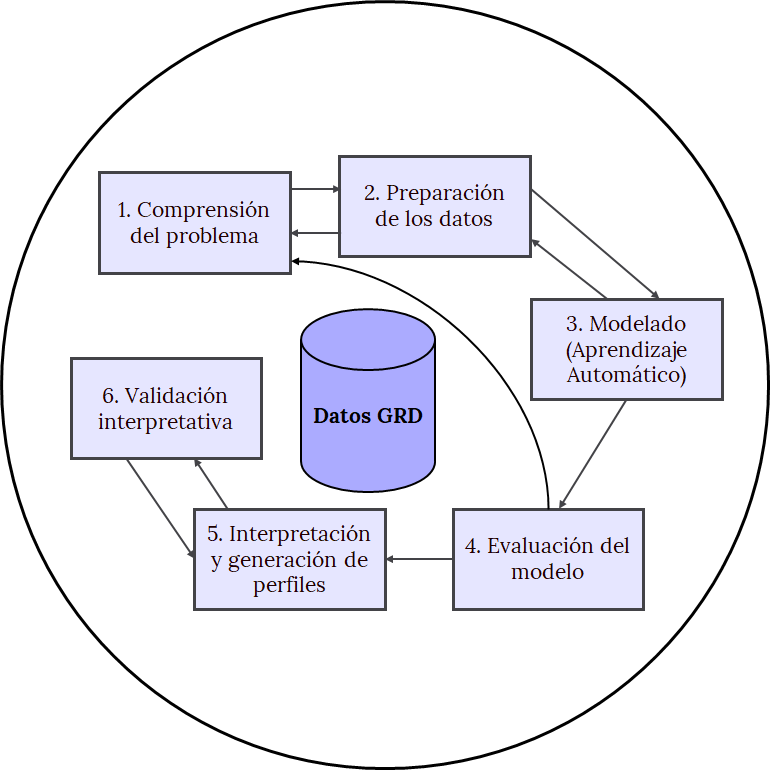
\includegraphics[width=0.5\textwidth]{images/figura1_seminario.png}

	\caption[Pipeline de trabajo propuesto (CRISP-DM) para el análisis.]{Pipeline de trabajo propuesto (CRISP-DM) para el análisis.\\Fuente: Elaboraci\'on propia, 2026.}
    \label{fig:metodologia_crisp_dm}
\end{figure}



Cabe mencionar que las seis fases oficiales de \textbf{CRISP-DM} son las siguientes:

\begin{enumerate}
\item \textbf{Comprensión del negocio o problema}.
\item \textbf{Comprensión de los datos}.
\item \textbf{Preparación de los datos}.
\item \textbf{Modelado}.
\item \textbf{Evaluación}.
\item \textbf{Despliegue}.
\end{enumerate}

Sin embargo, dado que esta propuesta no contempla la implementación de un software productivo, sino la generación de conocimiento analítico, la fase de \textbf{despliegue} fue adaptada y desglosada en las fases de \textbf{interpretación} y \textbf{validación interpretativa}. Por otro lado, la Figura \ref{fig:metodologia_crisp_dm} contempla flujos de retroalimentación críticos destinados a asegurar la calidad y consistencia metodológica de la solución:

\begin{itemize}

\item \textbf{De preparación a comprensión (Fase 2 $\rightarrow$ Fase 1):} este flujo permite validar tempranamente la viabilidad técnica de los objetivos planteados. Por ejemplo, si durante la exploración de datos se detectan limitaciones críticas, como variables con más del 30\% de valores nulos, inconsistencias temporales (por ejemplo, fechas de alta anteriores a la fecha de ingreso) o variables con un desbalance de clases extremadamente elevado (superior al 90\%), será necesario regresar a la fase 1 para realizar ajustes acotados en la definición de las variables objetivo o de entrada, garantizando así que el problema formulado sea técnicamente viable con los datos disponibles. Por ejemplo, si la variable de previsión de salud presenta valores nulos en el 99\% de los registros, resultaría inviable utilizarla como predictor, debiendo redefinirse las variables consideradas en la Fase 1.

\item \textbf{De modelado a preparación (Fase 4 $\rightarrow$ Fase 3):} este constituye el ciclo iterativo más frecuente, ya que, si los modelos aplicados (como Random Forest o XGBoost) obtienen un desempeño insuficiente (por ejemplo, un F1-Score inferior a 0,6), será necesario regresar a la fase de preparación para reprocesar los datos y experimentar con nuevas estrategias de imputación, transformación o balanceo de clases. Por ejemplo, si el modelo XGBoost evidencia un sobreajuste severo (\textit{overfitting}), se retornará a la Fase 3 para aplicar una ingeniería de características más agresiva, como agrupar códigos CIE-10 en categorías diagnósticas más generales, reduciendo así la dimensionalidad y favoreciendo la capacidad de generalización del modelo.

\item \textbf{De evaluación a comprensión (Fase 5 $\rightarrow$ Fase 1):} este flujo representa un mecanismo de contingencia frente a resultados no concluyentes. Si, tras la evaluación final, los modelos no alcanzan los umbrales de rendimiento esperados o presentan métricas anómalas (por ejemplo, un AUC-ROC igual a 1), el trabajo realizado no será descartado. En su lugar, se regresará a la Fase 1 para recalibrar los criterios de éxito, siempre que los resultados se mantengan dentro de un margen de tolerancia del 15\% respecto de los umbrales definidos inicialmente. En caso contrario, se documentará la inviabilidad predictiva como un hallazgo relevante acerca de las limitaciones actuales de los registros GRD, sin necesidad de reiniciar la investigación desde cero.

\item \textbf{De validación a interpretación (Fase 6 $\rightarrow$ Fase 5):} este flujo ocurre cuando los perfiles de riesgo obtenidos son matemáticamente consistentes, pero clínicamente redundantes debido a la presencia de variables dominantes. Por ejemplo, si en el análisis SHAP la variable más influyente corresponde al tipo de cáncer, esta podría aportar un valor limitado para la gestión hospitalaria en comparación con el conocimiento clínico ya existente. En dicho escenario, se regresará a la fase de interpretación para activar un protocolo de \textbf{análisis estratificado}, generando explicaciones SHAP específicas para distintos subgrupos diagnósticos.

\end{itemize}


\subsection{Herramientas de desarrollo}
Para la ejecución de los scripts de procesamiento de datos, modelado, evaluación y explicabilidad, se utilizará un computador de escritorio con sistema operativo Windows 10 de 64 bits, cuyas características principales son las siguientes:
\begin{itemize}

\item \textbf{Procesador (CPU):} AMD Ryzen 5 5500 @ 3.60 GHz, con 6 núcleos y 12 hilos de procesamiento lógico, lo que permitirá paralelizar el entrenamiento de algoritmos de ensamble, como Random Forest.

\item \textbf{Memoria RAM:} 16 GB DDR4 a 2667 MHz, capacidad suficiente para cargar y manipular en memoria el conjunto de datos GRD de episodios oncológicos mediante estructuras de datos en \textit{Pandas}.

\item \textbf{Tarjeta gráfica (GPU):} NVIDIA GeForce RTX 3050 con 6 GB de VRAM, la cual permitirá habilitar aceleración por hardware mediante CUDA, tecnología soportada nativamente por la librería XGBoost. El uso de GPU se justifica por la necesidad de reducir los tiempos de entrenamiento asociados a la búsqueda de hiperparámetros (\textit{Grid Search}) sobre un conjunto de datos de alta dimensionalidad y volumen considerable (más de 270.000 instancias), donde la ejecución exclusiva en CPU podría resultar computacionalmente costosa.

\item \textbf{Almacenamiento:} unidades SSD con una capacidad total aproximada de 2 TB (Crucial BX500 y ADATA Legend 710), garantizando altas velocidades de lectura y escritura (I/O) para el procesamiento eficiente de los datos.

\end{itemize}


Adicionalmente, se utilizará \textbf{Overleaf} para la redacción de informes y entregables en formato LaTeX, \textbf{Visual Studio Code} como editor de código para el desarrollo y mantenimiento de los scripts, y \textbf{GitHub} como sistema de control de versiones, con el objetivo de mantener la trazabilidad de los cambios realizados durante el procesamiento y modelado de datos, asegurando así la reproducibilidad de los experimentos.

Respecto al ambiente de desarrollo, el software será implementado utilizando el lenguaje de programación \textbf{Python} (versión 3.9 o superior), seleccionado por constituir el estándar actual en ciencia de datos y por disponer de un ecosistema robusto de librerías orientadas al aprendizaje automático y a la inteligencia artificial explicable (XAI), como SHAP (\cite{raschka2020machine, molnar2020interpretable}).

El entorno de trabajo se configurará mediante la distribución \textbf{Anaconda}, utilizando \textbf{Jupyter Notebook} como interfaz de desarrollo interactivo para las distintas etapas del proyecto (preparación de datos, modelado, evaluación e interpretación). Esta elección se fundamenta en la naturaleza exploratoria de la metodología CRISP-DM, donde resulta necesario visualizar resultados intermedios y facilitar tanto la depuración técnica como el análisis clínico de los hallazgos.

Las principales librerías y dependencias técnicas a utilizar serán las siguientes, las cuales están detalladas en la Tabla \ref{tab:librerias}:

\begin{itemize}
\item \textbf{Pandas y NumPy:} utilizadas para la manipulación matricial, estructuración de bases de datos, limpieza de registros y análisis exploratorio inicial.
\item \textbf{Scikit-Learn:} empleada para el escalamiento de datos, partición aleatoria de conjuntos, cálculo de métricas estadísticas y entrenamiento de modelos de clasificación tradicionales, como Random Forest y regresión logística.
\item \textbf{XGBoost y LightGBM:} frameworks de aprendizaje automático basados en \textit{Gradient Boosting}, utilizados por su alta eficiencia computacional y capacidad para capturar relaciones no lineales complejas presentes en los datos GRD.
\item \textbf{SHAP:} herramienta matemática basada en teoría de juegos que permite otorgar explicabilidad local y global a modelos de caja negra, cuantificando la contribución marginal de cada variable sobre las predicciones generadas.
\item \textbf{Matplotlib y Seaborn:} librerías utilizadas para la generación de visualizaciones estadísticas, matrices de correlación y gráficos de resumen asociados a los valores SHAP.
\end{itemize}


\begin{table}[htbp]
\centering
\footnotesize
\setlength{\tabcolsep}{4pt}
\renewcommand{\arraystretch}{1.15}
\caption{Librerías y dependencias del proyecto.}
\label{tab:librerias}
\begin{tabular}{|l|l|l|}
\hline
\parbox[t]{4.0cm}{\textbf{Librería (versión)}} & \parbox[t]{3.0cm}{\textbf{Propósito}} & \parbox[t]{8.0cm}{\textbf{Justificación en el proyecto}} \\ \hline
\parbox[t]{4.0cm}{\textbf{Pandas (v2.0+) / NumPy (v1.24+)}} & \parbox[t]{3.0cm}{Manipulación de datos} & \parbox[t]{8.0cm}{Se usarán para el procesamiento vectorial de los registros GRD y el manejo eficiente de estructuras de datos tabulares (DataFrames), aprovechando el soporte nativo para tipos de datos nulos de las versiones recientes (\cite{mckinney2010pandas}).} \\ \hline
\parbox[t]{4.0cm}{\textbf{Matplotlib (v3.7+) / Seaborn (v0.12+)}} & \parbox[t]{3.0cm}{Visualización} & \parbox[t]{8.0cm}{Se usarán para la generación de gráficos estáticos de alta calidad para el Análisis Exploratorio de Datos (EDA) y para reportes visuales de resultados (como matrices de confusión) (\cite{hunter2007matplotlib}).} \\ \hline
\parbox[t]{4.0cm}{\textbf{Scikit-learn (v1.3+)}} & \parbox[t]{3.0cm}{Modelado base} & \parbox[t]{8.0cm}{Para la implementación de algoritmos clásicos (regresión logística, Random Forest), técnicas de preprocesamiento (One-Hot Encoding, imputación) y el cálculo de métricas de evaluación (\cite{pedregosa2011scikit}).} \\ \hline
\parbox[t]{4.0cm}{\textbf{XGBoost (v2.0+)}} & \parbox[t]{3.0cm}{Modelado avanzado} & \parbox[t]{8.0cm}{Implementación del algoritmo de \textit{Gradient Boosting} optimizado. Se selecciona esta versión por su soporte mejorado para aceleración por GPU y el manejo nativo de valores faltantes (\cite{chen2016xgboost}).} \\ \hline
\parbox[t]{4.0cm}{\textbf{SHAP (v0.42+)}} & \parbox[t]{3.0cm}{Explicabilidad (XAI)} & \parbox[t]{8.0cm}{Cálculo de valores de Shapley para interpretar modelos de caja negra (Random Forest, XGBoost), permitiendo extraer reglas de decisión globales y locales consistentes (\cite{lundberg2017shap}).} \\ \hline
\parbox[t]{4.0cm}{\textbf{Imbalanced-learn (v0.12+)}} & \parbox[t]{3.0cm}{Balanceo de datos} & \parbox[t]{8.0cm}{Librería auxiliar que proporciona técnicas de remuestreo (SMOTE) para manejar el desbalance severo de clases, compatible con las versiones recientes de Scikit-learn (\cite{lemaitre2017imbalanced}).} \\ \hline
\end{tabular}
\end{table}

\section{Organizaci\'on del documento}
\label{intro:organizacion}
El presente documento se estructura en cinco capítulos, los cuales guían de manera progresiva y sistemática el desarrollo de la investigación orientada a la caracterización descriptiva de episodios oncológicos en la red pública de salud chilena. A continuación, se detalla brevemente el propósito y contenido de cada apartado:

\begin{itemize}

\item \textbf{Capítulo 1 - Introducción:} establece el marco inicial del estudio mediante la descripción del contexto epidemiológico y operativo del cáncer en Chile, así como de la implementación institucional del sistema de Grupos Relacionados por el Diagnóstico (GRD). En esta sección se define el problema de investigación, formulando la pregunta de investigación, la hipótesis de trabajo, los objetivos generales y específicos, las delimitaciones del alcance y una síntesis de la metodología y herramientas de desarrollo a utilizar.

\item \textbf{Capítulo 2 - Antecedentes:} aborda la revisión del estado del arte y el sustento teórico de la investigación. En esta sección se presentan los fundamentos clínicos de las neoplasias malignas y los mecanismos operativos del estándar International Refined (IR-GRD) bajo la administración de FONASA. Adicionalmente, se examina literatura científica nacional e internacional relacionada con el uso de registros clínico-administrativos masivos, técnicas estadísticas para el análisis de asociaciones no lineales y fundamentos matemáticos de la Inteligencia Artificial Explicable (XAI).

\item \textbf{Capítulo 3 - Metodología:} expone el diseño experimental e investigativo basado en una adaptación del ciclo de vida CRISP-DM. Se detalla el proceso de extracción, análisis de variables numéricas y categóricas, limpieza, transformación, derivación y codificación bivariada de la base de datos histórica correspondiente al período 2019--2024, incorporando tanto la cohorte oncológica como la cohorte de control (sin cáncer). Además, se describe el entrenamiento de modelos, la optimización de hiperparámetros mediante \textit{Grid Search} y validación cruzada, la implementación de remuestreo iterativo (\textit{bootstrapping}) para medir la estabilidad de las variables, la evaluación de los modelos sobre el conjunto de prueba y la extracción de valores SHAP para la interpretación direccional de cada desenlace de riesgo.

\item \textbf{Capítulo 4 - Resultados y análisis:} presenta los hallazgos empíricos derivados del flujo analítico desarrollado, incluyendo la identificación y jerarquización de las variables estadísticamente más relevantes en los episodios hospitalarios, así como la visualización cuantitativa de los impactos locales y globales de cada atributo sobre las variables objetivo mediante SHAP. El análisis considera tanto la discriminación basal entre pacientes con cáncer y sin cáncer como la caracterización específica de los distintos perfiles oncológicos. Finalmente, los resultados son discutidos críticamente, contrastando las reglas de asociación identificadas con la práctica médica oncológica y la realidad de la gestión sanitaria pública.

\item \textbf{Capítulo 5 - Conclusiones:} sintetiza las conclusiones generales del estudio en función del cumplimiento de los objetivos planteados y de la validación de la hipótesis de trabajo. Asimismo, se destacan las principales contribuciones metodológicas derivadas del uso descriptivo de modelos avanzados aplicados sobre datos administrativos en Chile, se exponen de manera transparente las limitaciones conceptuales y técnicas de los registros GRD, y se proponen futuras líneas de investigación orientadas al diseño de políticas de planificación hospitalaria basadas en evidencia.

\end{itemize}